% !TeX program = xelatex
\documentclass[12pt,a4paper]{article}
\usepackage{fontspec}
\setmainfont{Times New Roman}
\setsansfont{Arial}
\setmonofont{Consolas}
\usepackage{polyglossia}
\setdefaultlanguage{russian}
\setotherlanguage{english}
\usepackage{amsmath,amssymb}
\usepackage[a4paper,margin=20mm,top=18mm,bottom=20mm]{geometry}
\usepackage{graphicx,booktabs,longtable,array}
\usepackage{caption}
\captionsetup{font=small,labelfont=bf,labelsep=period}
\usepackage{fvextra}
\usepackage[hidelinks]{hyperref}
\hypersetup{pdftitle={Вычислительная математика. ДЗ 1. Вариант 25},pdfauthor={Тимофей Рыко}}
\setlength{\parindent}{1.25cm}
\setlength{\parskip}{3pt}
\setlength{\emergencystretch}{2em}
\linespread{1.08}
\allowdisplaybreaks
\AtBeginDocument{\setlength{\abovedisplayskip}{8pt}\setlength{\belowdisplayskip}{8pt}}
\pagestyle{plain}
\title{\textbf{Вычислительная математика}\\[6pt]Домашнее задание № 1\\Вариант 25}
\author{Тимофей Рыко}
\date{17 октября 2026 года}
\begin{document}
\begin{center}
{\large\bfseries Вычислительная математика}\\[4pt]
{\large Домашнее задание № 1. Вариант 25}\\[6pt]
Тимофей Рыко\\[2pt]
17 октября 2026 года
\end{center}
\section{Что требуется сделать}
Для двух функций нужно построить интерполяционный полином и кубический сплайн. В каждом случае берутся от 20 до 60 узлов: сначала равномерных, затем чебышёвских. Нужно сравнить точность методов, получить оценки ошибки и проверить влияние чётности степени полинома.

\[
f_1(x)=\cos x,\quad x\in[0,2\pi];\qquad f_2(x)=\tanh x,\quad x\in[-\pi,\pi].
\]
\textbf{Интерполяция} означает, что построенная функция точно совпадает с исходной во всех выбранных узлах. Между узлами они могут различаться. Эти различия и исследуются в работе.

\subsection{Какие узлы используются}
N — число узлов. Полином через N точек имеет степень не выше N-1. Например, при N=20 его степень не выше 19. Пусть [a,b] — заданный отрезок, L=b-a=2\ensuremath{\pi}.

\textbf{Равномерная сетка:} расстояния между соседними узлами одинаковы, крайние узлы совпадают с a и b.

\[
x_j=a+\frac{j(b-a)}{N-1},\qquad j=0,\ldots,N-1.
\]
\textbf{Сетка Чебышёва:} узлы сгущены к концам отрезка. По условию используются нули полинома Чебышёва T\textsubscript{N}:

\[
x_j=\frac{a+b}{2}+\frac{b-a}{2}\cos\frac{(2j+1)\pi}{2N},\qquad j=0,\ldots,N-1.
\]
Эти узлы не включают сами концы отрезка. Перед расчётом они сортируются по возрастанию. В обоих случаях узлов ровно N.

\subsection{Как сравнивается точность}
В каждой точке берётся модуль разности исходной функции и приближения. Затем находится наибольшее значение на всём заданном отрезке:

\[
E_P=\max_{[a,b]}|f(x)-P(x)|,\qquad E_S=\max_{[a,b]}|f(x)-S(x)|.
\]
P обозначает полином, S — сплайн. Чем меньше E, тем точнее приближение. В таблицах максимум найден численно. Априорная оценка B — это выведенная из формул верхняя граница: ошибка должна удовлетворять E\ensuremath{\leq}B.

\clearpage
\section{Интерполяционный полином}
Через N различных узлов проходит единственный полином степени не выше N-1. Для расчёта выбрана форма Ньютона:

\[
P(x)=c_0+\sum_{k=1}^{N-1}c_k\prod_{j=0}^{k-1}(x-x_j).
\]
Коэффициенты c\textsubscript{k} — разделённые разности. Начальный столбец состоит из значений функции. Каждый следующий получается вычитанием соседних элементов и делением на расстояние между крайними узлами:

\[
f[x_i,\ldots,x_{i+k}]=\frac{f[x_{i+1},\ldots,x_{i+k}]-f[x_i,\ldots,x_{i+k-1}]}{x_{i+k}-x_i}.
\]
Значение полинома считается вложенным умножением, как в схеме Горнера. Решать большую систему для коэффициентов при степенях x не требуется.

\subsection{Оценка погрешности}
Если у функции есть непрерывная производная порядка N, остаток интерполяции имеет вид:

\[
f(x)-P(x)=\frac{f^{(N)}(\xi)}{N!}\prod_{j=0}^{N-1}(x-x_j),\qquad \xi\in[a,b].
\]
Пусть M\textsubscript{N} — верхняя граница модуля этой производной. Обозначим произведение расстояний до узлов через \ensuremath{\omega}\textsubscript{N}. Тогда:

\[
E_P\leq\frac{M_N}{N!}\max_{[a,b]}|\omega_N(x)|.
\]
\textbf{Равномерная сетка.} При шаге h=L/(N-1) произведение расстояний до двух ближайших узлов не больше h\textsuperscript{2}/4. Остальные множители можно ограничить последовательными кратными h. Отсюда:

\[
\max|\omega_N|\leq\frac{h^N(N-1)!}{4},\qquad B_P=\frac{M_Nh^N}{4N}.
\]
\textbf{Нули Чебышёва.} Здесь \ensuremath{\omega}\textsubscript{N} пропорционально T\textsubscript{N}, а |T\textsubscript{N}|\ensuremath{\leq}1 на [-1,1]. С учётом длины отрезка:

\[
\max|\omega_N|=2\left(\frac{L}{4}\right)^N,\qquad B_P=\frac{2M_N}{N!}\left(\frac{L}{4}\right)^N.
\]
На следующей странице показано, как получить M\textsubscript{N} для обеих функций. Эти оценки относятся к самому полиному. Погрешность округления компьютера рассматривается отдельно.

\clearpage
\section{Как оцениваются производные}
\subsection{Функция cos x}
Производные cos x последовательно равны -sin x, -cos x, sin x, cos x и затем повторяются. Их модуль не больше 1. Поэтому для любого N можно взять \textbf{M\textsubscript{N}=1} и подставить его в формулы предыдущей страницы.

\subsection{Функция tanh x}
Чтобы не выписывать вручную производные до 60-го порядка, используется простое рекуррентное правило. Положим t=tanh x. Тогда t\ensuremath{\prime}=1-t\textsuperscript{2}, поэтому каждая производная tanh x является полиномом от t:

\[
Q_0(t)=t,\qquad Q_{k+1}(t)=(1-t^2)Q_k^{\prime}(t),\qquad f^{(k)}(x)=Q_k(\tanh x).
\]
Например, первые два шага дают:

\[
Q_1(t)=1-t^2,\qquad Q_2(t)=-2t+2t^3.
\]
Так как |tanh x|\ensuremath{\leq}1, модуль каждого t\textsuperscript{j} также не больше 1. Следовательно, модуль полинома не превышает сумму модулей его коэффициентов:

\[
Q_N(t)=\sum_j a_jt^j\quad\Longrightarrow\quad |f^{(N)}(x)|\leq\sum_j|a_j|=:M_N.
\]
Программа строит коэффициенты Q\textsubscript{N} по указанному правилу. Они целые, поэтому эта часть расчёта выполняется без округления. Полученное M\textsubscript{N} подставляется в оценки для обеих сеток.

\textbf{Почему оценка может быть большой?} При суммировании модулей теряется взаимное сокращение слагаемых. Поэтому такая граница для tanh x сильно завышена. Она подходит для проверки E\ensuremath{\leq}B, но по ней нельзя судить, сходится ли интерполяция. Большая верхняя граница не означает большую фактическую ошибку.

\subsection{Что означает чётность степени}
В задании степень удобно обозначать n=N-1. Но это верхняя граница: некоторые старшие коэффициенты могут оказаться нулевыми. На симметричной сетке полином сохраняет симметрию функции. Поэтому полином для cos x чётен относительно центра \ensuremath{\pi}, а для tanh x нечётен относительно нуля.

При сравнении чётности используются соседние пары N=20 и 21, 22 и 23, \ldots{}, 58 и 59. Это позволяет видеть влияние чётности отдельно от общего увеличения числа узлов. Результаты для разных сеток рассматриваются отдельно.

\clearpage
\section{Кубический сплайн}
Полином строится сразу на всём отрезке. Сплайн устроен иначе: между каждой парой соседних узлов строится свой кубический полином. В узлах соседние части соединяются так, чтобы совпадали значение, первая и вторая производные.

Используется \textbf{естественный кубический сплайн}, как в семинаре 6: на краях сетки его вторая производная равна нулю. Это выбранные граничные условия для сплайна Шёнберга.

\[
S(x_i)=f(x_i),\qquad S\in C^2,\qquad S^{\prime\prime}(x_0)=S^{\prime\prime}(x_{N-1})=0.
\]
Пусть h\textsubscript{i}=x\textsubscript{i+1}-x\textsubscript{i}, y\textsubscript{i}=f(x\textsubscript{i}), m\textsubscript{i}=S\ensuremath{\prime\prime}(x\textsubscript{i}). Неизвестные вторые производные находятся из системы для i=1,\ldots{},N-2:

\[
\begin{aligned}&h_{i-1}m_{i-1}+2(h_{i-1}+h_i)m_i+h_im_{i+1}\\ &=6\left(\frac{y_{i+1}-y_i}{h_i}-\frac{y_i-y_{i-1}}{h_{i-1}}\right).\end{aligned}
\]
После этого кубический участок определяется однозначно. Если u=(x-x\textsubscript{i})/h\textsubscript{i}, а L\textsubscript{i} — прямая между соседними значениями функции, то:

\[
S(x)=L_i(x)+\frac{h_i^2}{6}\left[m_i((1-u)^3-(1-u))+m_{i+1}(u^3-u)\right].
\]
\textbf{На сетке Чебышёва} крайние узлы не совпадают с концами отрезка. На оставшихся коротких участках сплайн продолжается касательными прямыми. Например, слева S(x)=S(x\textsubscript{0})+S\ensuremath{\prime}(x\textsubscript{0})(x-x\textsubscript{0}). Новые узлы не добавляются; значение и первые две производные остаются непрерывными.

\subsection{Оценка погрешности сплайна}
Обозначим H=max h\textsubscript{i} и M\textsubscript{2}=max|f\ensuremath{\prime\prime}|. Из системы для m\textsubscript{i} получается max|m\textsubscript{i}|\ensuremath{\leq}3M\textsubscript{2}: диагональный коэффициент вдвое больше суммы соседних, а правая часть ограничена через M\textsubscript{2}. Ошибка прямой L\textsubscript{i} не больше M\textsubscript{2}h\textsubscript{i}\textsuperscript{2}/8, отличие сплайна от этой прямой — не больше 3M\textsubscript{2}h\textsubscript{i}\textsuperscript{2}/8. Складывая, получаем:

\[
E_S\leq\frac{M_2H^2}{2}\qquad\text{между крайними узлами}.
\]
Для линейного продолжения на длину \ensuremath{\delta} слева добавляется граница M\textsubscript{2}(\ensuremath{\delta}h\textsubscript{0}+\ensuremath{\delta}\textsuperscript{2}/2), справа — аналогичная. В программе B\textsubscript{S} равна максимуму внутренней и двух крайних границ.

\[
M_2(\cos)=1,\qquad M_2(\tanh)=\frac{4}{3\sqrt{3}}.
\]
Последнее значение получается из f\ensuremath{\prime\prime}=-2t(1-t\textsuperscript{2}), t=tanh x: максимум модуля достигается при |t|=1/\ensuremath{\surd}3. Полученная оценка имеет порядок H\textsuperscript{2}. Обещать порядок H\textsuperscript{4} на всём отрезке здесь нельзя: естественные условия S\ensuremath{\prime\prime}=0 не совпадают с f\ensuremath{\prime\prime} на краях.

\clearpage
\section{Как выполнен расчёт}
\textbf{1. Построение.} Для каждого N от 20 до 60 строятся обе сетки. В узлах вычисляются cos x или tanh x. По этим значениям строятся полином Ньютона и естественный сплайн. Всего получается 164 набора данных и 328 приближений.

\textbf{2. Поиск ошибки.} Приближения сравниваются с исходной функцией на объединении двух проверочных сеток: 2001 равномерной точки и 2001 точки со сгущением к краям. Затем уточняется положение пяти наибольших локальных пиков ошибки. Концы исходного отрезка также проверяются.

\textbf{3. Почему повышена точность.} У cos x ошибка полинома становится намного меньше 10\textsuperscript{-16}. Обычная арифметика компьютера уже не позволяет её различить. Поэтому полином считается с 90 десятичными знаками. Каждый найденный максимум дополнительно проверяется другой формой того же полинома при 120 знаках.

\textbf{4. Проверки.} Подтверждено совпадение приближений с функцией в узлах, выполнение условий S\ensuremath{\prime\prime}=0 и неравенств E\ensuremath{\leq}B. Для N=20,21,40,41,59,60 расчёт дополнительно проверен на сетке из 8001 точки. Существенно больших ошибок на ней не найдено. Табличный максимум остаётся численной оценкой, а не точным аналитическим значением.

\subsection{Ошибка полинома и ошибка округления}
\begin{center}\small\setlength{\tabcolsep}{5pt}\renewcommand{\arraystretch}{1.18}
\begin{tabular}{rrrr}\toprule
cos x, N & Сетка & Ошибка P, 90 знаков & \shortstack{Ошибка\\расчёта float64}\\ \midrule
20 & равномерная & 1.077e-12 & 1.750e-12\\
20 & Чебышёв & 6.178e-15 & 6.772e-15\\
40 & равномерная & 3.799e-35 & 5.676e-07\\
40 & Чебышёв & 1.619e-40 & 7.772e-16\\
60 & равномерная & 5.357e-62 & 4.931e-01\\
60 & Чебышёв & 1.352e-70 & 9.992e-16\\
\bottomrule\end{tabular}\end{center}
Float64 — обычные вычисления примерно с 16 значащими десятичными цифрами. В последнем столбце приведена ошибка библиотечного барицентрического интерполятора SciPy на проверочной сетке.

На равномерной сетке при большом N даже малые округления узлов и значений сильно влияют на результат. Поэтому при N=60 обычный расчёт cos x ошибается почти на 0,5, хотя сам интерполяционный полином очень точен. На сетке Чебышёва округление ограничивает результат уровнем около 10\textsuperscript{-15}. Основные таблицы ниже содержат высокоточные полиномиальные результаты.

Сплайн считается обычной арифметикой: его ошибки здесь достаточно велики, чтобы надёжно отличаться от округления.

\clearpage
\section{Результаты для cos x}
\begin{figure}[!htbp]
\centering
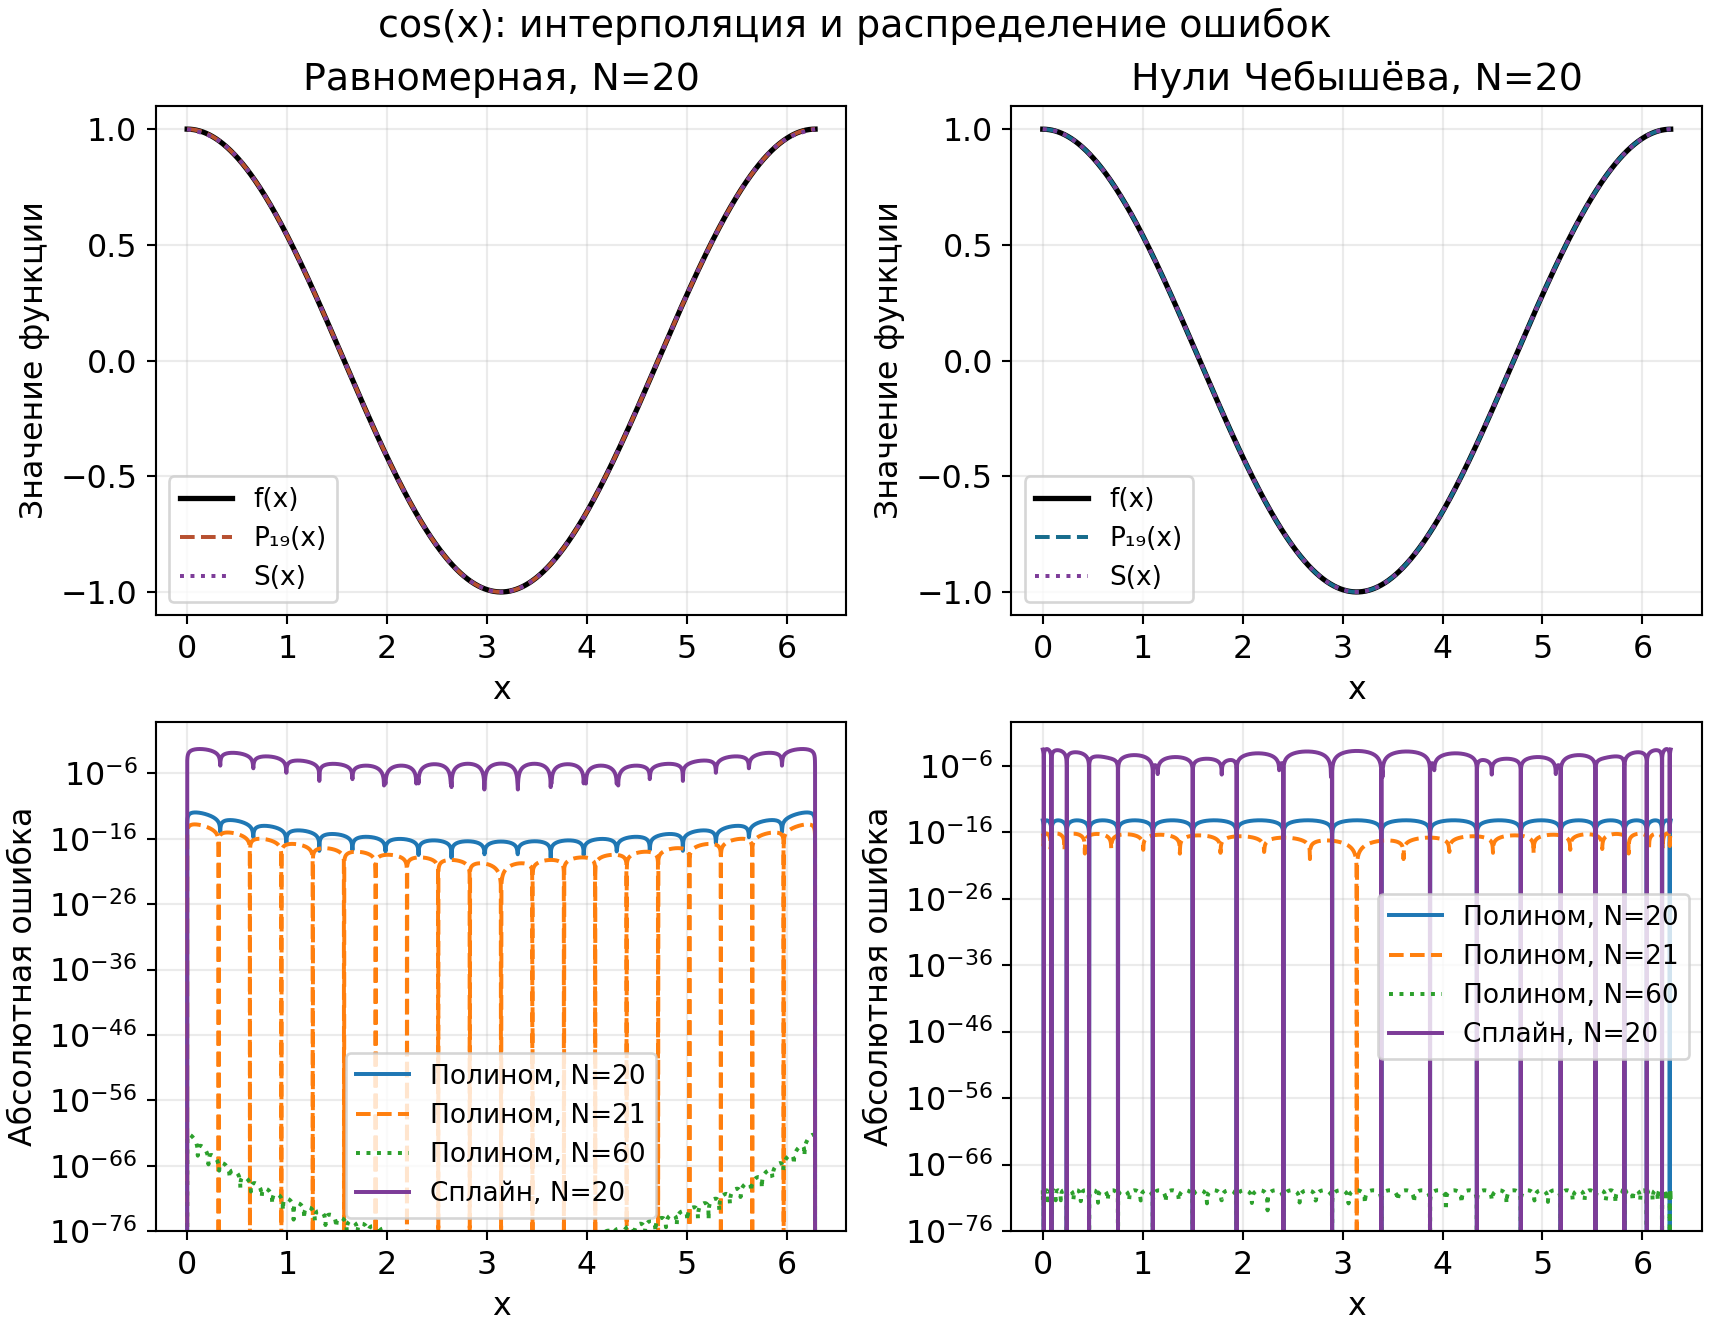
\includegraphics[width=\linewidth]{images/cos_curves.png}
\caption{Сверху — функция, полином и сплайн при N=20. Снизу — абсолютные ошибки. По вертикали в нижних графиках логарифмическая шкала: каждый следующий порядок означает изменение ошибки в 10 раз.}
\end{figure}
\begin{center}\small\setlength{\tabcolsep}{5pt}\renewcommand{\arraystretch}{1.18}
\begin{tabular}{rrrrr}\toprule
N & P: равномерная & P: Чебышёв & S: равномерная & S: Чебышёв\\ \midrule
20 & 1.077e-12 & 6.178e-15 & 5.446e-03 & 3.204e-04\\
21 & 1.611e-14 & 6.566e-17 & 4.908e-03 & 2.638e-04\\
40 & 3.799e-35 & 1.619e-40 & 1.279e-03 & 2.020e-05\\
41 & 1.562e-37 & 4.634e-43 & 1.215e-03 & 1.830e-05\\
59 & 7.321e-62 & 2.699e-70 & 5.770e-04 & 4.275e-06\\
60 & 5.357e-62 & 1.352e-70 & 5.576e-04 & 3.997e-06\\
\bottomrule\end{tabular}\end{center}
Полином быстро приближает cos x на обеих сетках. При N=60 чебышёвские узлы дают ошибку 1,352\ensuremath{\cdot}10\textsuperscript{-70}, равномерные — 5,357\ensuremath{\cdot}10\textsuperscript{-62}. На верхних графиках полином практически совпадает с функцией; разницу показывает график ошибки.

Сплайн менее точен. Его наибольшая ошибка на равномерной сетке возникает около концов: у cos x там f\ensuremath{\prime\prime}=-1, а у естественного сплайна S\ensuremath{\prime\prime}=0. Чебышёвские узлы расположены плотнее у границ и уменьшают эту ошибку. При N=60 такой сплайн примерно в 140 раз точнее равномерного.

\clearpage
\subsection{cos x: оценки и чётность}
\begin{figure}[!htbp]
\centering
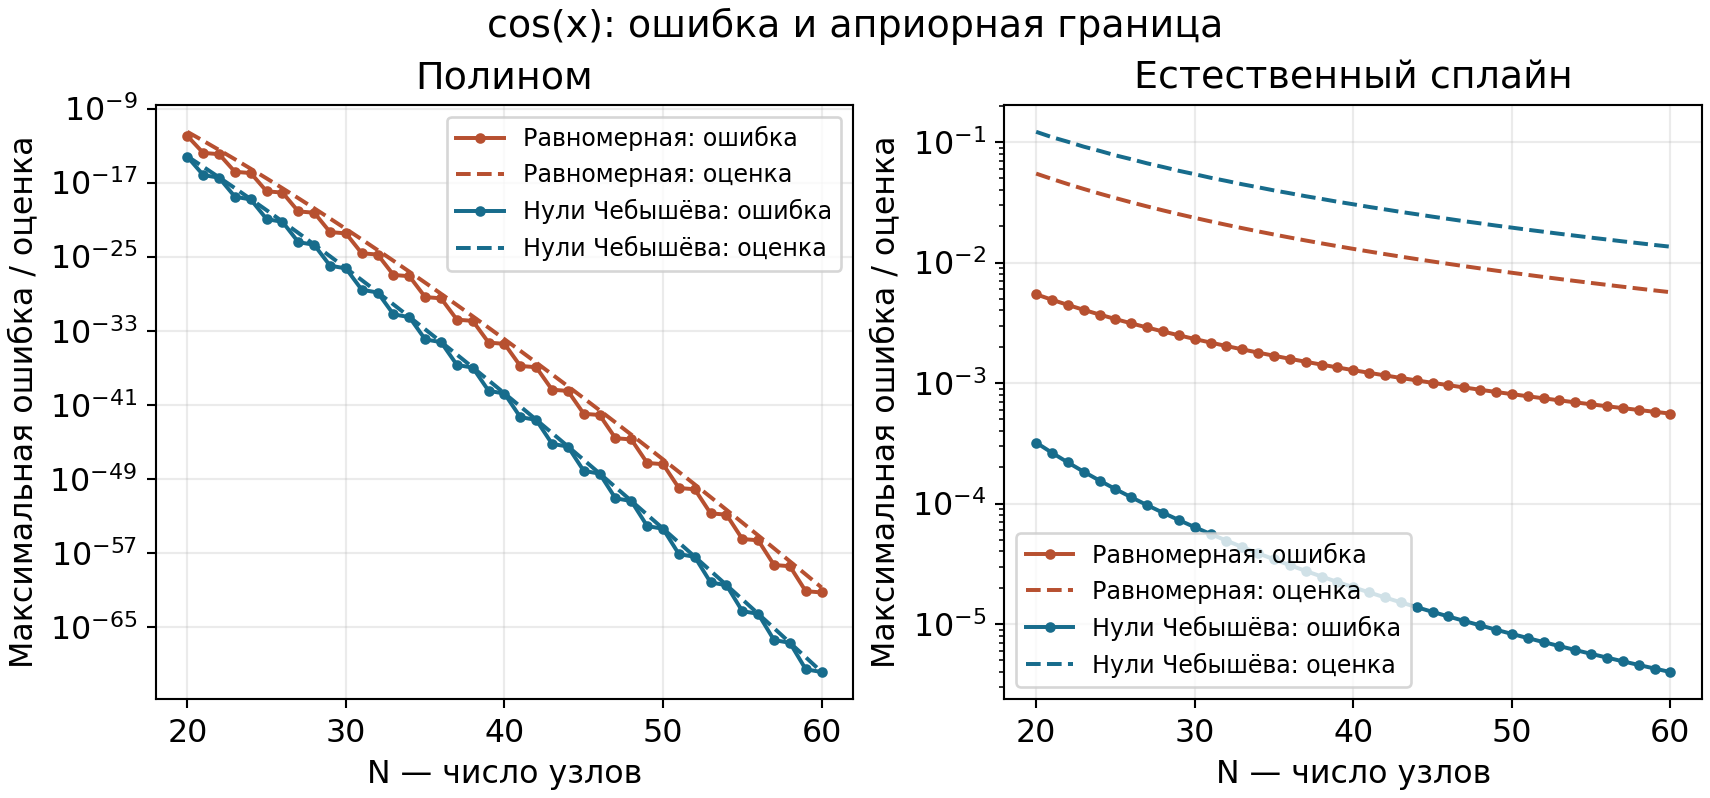
\includegraphics[width=\linewidth]{images/cos_convergence.png}
\caption{Ошибка при всех N от 20 до 60 и её априорная граница. Сплошная линия — ошибка, пунктирная — граница. Чем ниже линия, тем меньше соответствующая величина.}
\end{figure}
\begin{center}\small\setlength{\tabcolsep}{5pt}\renewcommand{\arraystretch}{1.18}
\begin{tabular}{rrrrrr}\toprule
N & Сетка & E\textsubscript{P} & B\textsubscript{P} & E\textsubscript{S} & B\textsubscript{S}\\ \midrule
20 & равн. & 1.077e-12 & 3.058e-12 & 5.446e-03 & 5.468e-02\\
20 & Чеб. & 6.178e-15 & 6.875e-15 & 3.204e-04 & 1.215e-01\\
60 & равн. & 5.357e-62 & 1.817e-61 & 5.576e-04 & 5.671e-03\\
60 & Чеб. & 1.352e-70 & 1.406e-70 & 3.997e-06 & 1.353e-02\\
\bottomrule\end{tabular}\end{center}
Все ошибки ниже соответствующих границ. Для полинома при N=60 на сетке Чебышёва оценка завышает ошибку всего примерно на 4\%. Оценка сплайна заметно грубее, поскольку использует только максимальный шаг и не учитывает, где именно сгущены узлы.

\textbf{Влияние чётности.} Относительно центра \ensuremath{\pi} функция cos x чётна: cos(\ensuremath{\pi}+t)=-cos t. Интерполяционный полином тоже чётен по t. При N=20 разрешена степень до 19, но нечётный старший член равен нулю: фактическая степень не выше 18. При N=21 доступна степень 20. Поэтому переход 20\ensuremath{\to}21 резко улучшает точность. Следующий переход 21\ensuremath{\to}22 оставляет ту же доступную чётную степень 20.

Во всех соседних парах (20,21),\ldots{},(58,59) меньше ошибка у нечётного N на обеих сетках. То есть в обозначении n=N-1 предпочтительна \textbf{чётная степень}. Это сравнение соседних пар: оно не означает, что любое нечётное N лучше любого чётного.

\clearpage
\section{Результаты для tanh x}
\begin{figure}[!htbp]
\centering
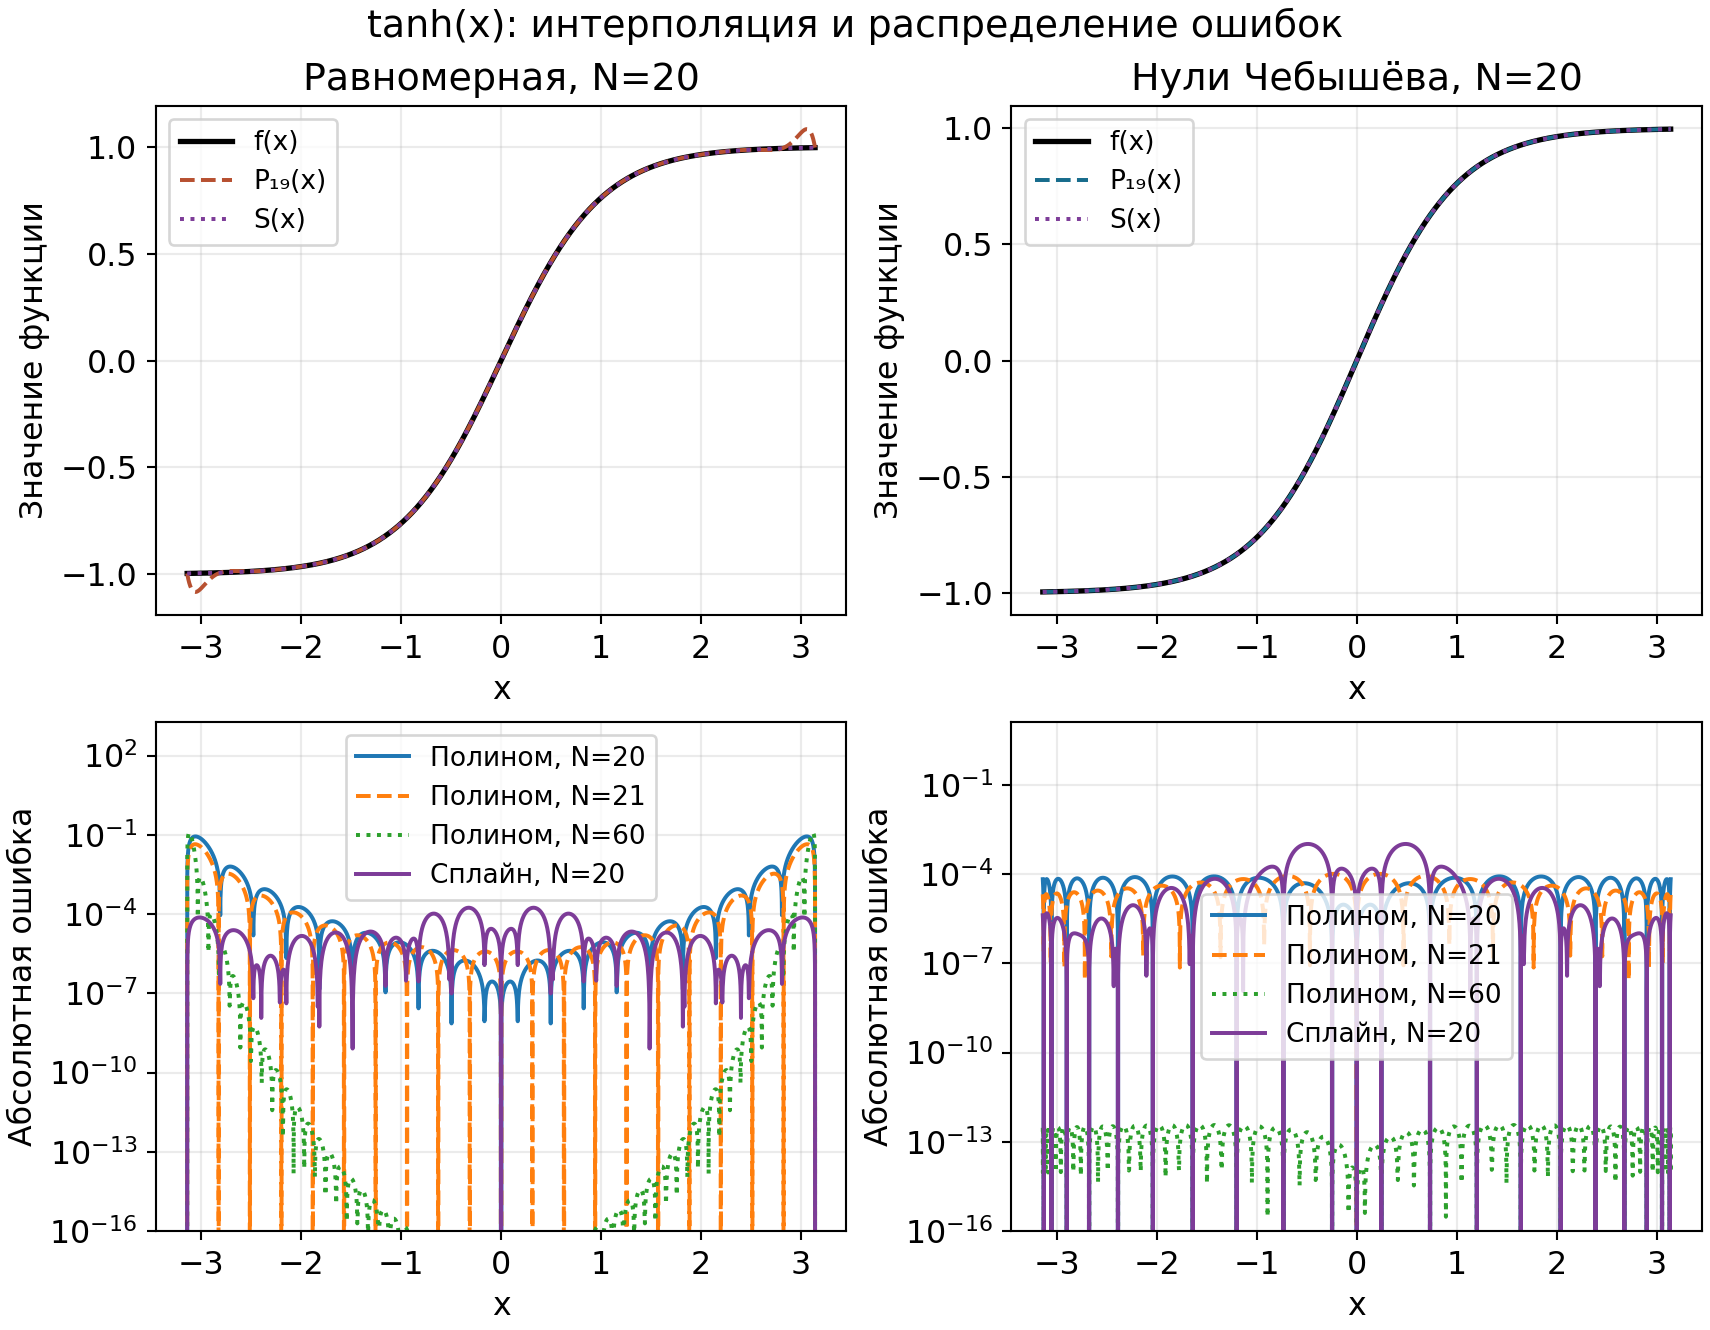
\includegraphics[width=\linewidth]{images/tanh_curves.png}
\caption{Функция, приближения и абсолютные ошибки. У равномерного полинома заметны отклонения около концов отрезка. Чебышёвский полином приближает функцию всё точнее с ростом N.}
\end{figure}
\begin{center}\small\setlength{\tabcolsep}{5pt}\renewcommand{\arraystretch}{1.18}
\begin{tabular}{rrrrr}\toprule
N & P: равномерная & P: Чебышёв & S: равномерная & S: Чебышёв\\ \midrule
20 & 8.726e-02 & 8.378e-05 & 1.744e-04 & 1.030e-03\\
21 & 4.428e-02 & 1.018e-04 & 1.304e-04 & 8.405e-04\\
40 & 9.020e-02 & 5.559e-09 & 1.863e-05 & 4.189e-05\\
41 & 4.604e-02 & 6.838e-09 & 1.772e-05 & 4.107e-05\\
59 & 5.839e-02 & 1.187e-12 & 8.490e-06 & 8.706e-06\\
60 & 1.179e-01 & 3.678e-13 & 8.206e-06 & 7.938e-06\\
\bottomrule\end{tabular}\end{center}
На равномерной сетке увеличение числа узлов не решает проблему. Сначала ошибка немного снижается, затем растёт. Минимум среди чётных N достигается при N=28 (\ensuremath{\approx}0,0841), среди нечётных — при N=27 (\ensuremath{\approx}0,0428). При N=60 ошибка уже равна 0,1179. Такие краевые колебания полинома называют \textbf{эффектом Рунге}.

На сетке Чебышёва ошибка уменьшается до 3,678\ensuremath{\cdot}10\textsuperscript{-13}. Сплайны на обеих сетках также становятся точнее и при N=60 дают близкие ошибки около 8\ensuremath{\cdot}10\textsuperscript{-6}. При малом N равномерный сплайн лучше: в центральной области быстрого изменения tanh x у него больше узлов.

\clearpage
\subsection{tanh x: оценки и чётность}
\begin{figure}[!htbp]
\centering
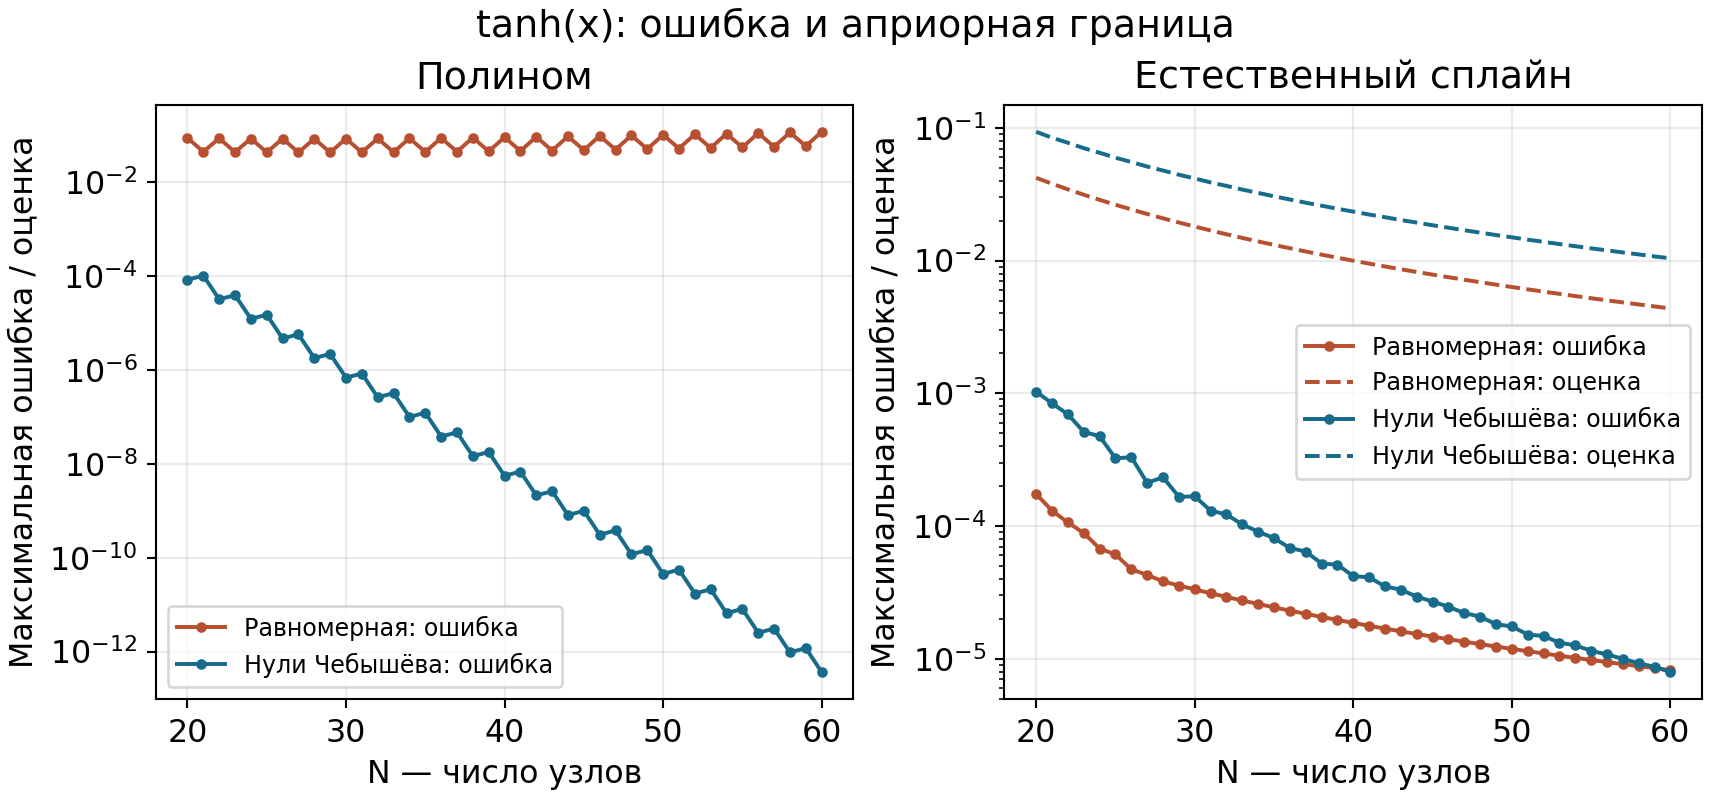
\includegraphics[width=\linewidth]{images/tanh_convergence.png}
\caption{Слева — ошибки полиномов, справа — ошибки сплайнов и их границы. Грубые оценки полиномиальной ошибки вынесены в таблицу: на общем графике их большие значения скрыли бы различия фактических ошибок.}
\end{figure}
\begin{center}\small\setlength{\tabcolsep}{5pt}\renewcommand{\arraystretch}{1.18}
\begin{tabular}{rrrrrr}\toprule
N & Сетка & E\textsubscript{P} & B\textsubscript{P} & E\textsubscript{S} & B\textsubscript{S}\\ \midrule
20 & равн. & 8.726e-02 & 1.188e+09 & 1.744e-04 & 4.209e-02\\
20 & Чеб. & 8.378e-05 & 2.670e+06 & 1.030e-03 & 9.354e-02\\
60 & равн. & 1.179e-01 & 3.794e+27 & 8.206e-06 & 4.365e-03\\
60 & Чеб. & 3.678e-13 & 2.936e+18 & 7.938e-06 & 1.041e-02\\
\bottomrule\end{tabular}\end{center}
Неравенства E\ensuremath{\leq}B выполнены, но полиномиальная оценка сильно завышена. Причина — грубая граница для высокой производной: сумма модулей коэффициентов не учитывает их сокращение. Поэтому эта оценка не объясняет хорошее поведение чебышёвского полинома. Оно установлено численным расчётом.

\textbf{Влияние чётности.} Функция tanh x нечётна, и её интерполяционный полином тоже нечётен. При N=20 и N=21 фактическая степень не выше 19 в обоих случаях. При этом узлы различаются, поэтому совпадения ошибок ожидать нельзя.

\textbf{Сетка Чебышёва:} во всех 20 парах (20,21),\ldots{},(58,59) лучше чётное N. Следовательно, в обозначении n=N-1 лучше \textbf{нечётная степень}. Например, при N=20 ошибка 8,378\ensuremath{\cdot}10\textsuperscript{-5}, при N=21 — 1,018\ensuremath{\cdot}10\textsuperscript{-4}.

\textbf{Равномерная сетка:} во всех тех же парах лучше нечётное N, то есть \textbf{чётная степень n=N-1}. Фактический полином при этом всё равно нечётный: коэффициент при старшей чётной степени равен нулю. Например, ошибки при N=20 и 21 равны 0,08726 и 0,04428. Значит, единого правила чётности для всех сеток здесь нет.

\clearpage
\section{Выводы}
\textbf{1. Для cos x полиномиальная интерполяция точнее сплайна.} Ошибка быстро уменьшается на обеих сетках, особенно на чебышёвской. Но для больших N нужны вычисления с повышенной точностью, иначе результат искажает округление.

\textbf{2. Для tanh x важно выбрать правильную сетку.} Равномерный полином имеет краевые колебания, которые не исчезают при увеличении N до 60. Чебышёвская сетка даёт быстрое уменьшение ошибки: при N=60 она около 3,68\ensuremath{\cdot}10\textsuperscript{-13}.

\textbf{3. Сплайн даёт устойчивый результат для обеих функций.} Он уступает хорошему полиному по точности, но не испытывает сильных краевых колебаний высокой степени. Его ошибка зависит от граничных условий. Для cos x сгущение узлов у концов заметно улучшает результат.

\textbf{4. Априорная оценка — это граница, а не прогноз точного значения.} Для cos x остаточная оценка полинома достаточно близка к ошибке. Для tanh x применённая простая оценка производной сильно завышает её. Все проверенные ошибки находятся ниже выведенных границ.

\textbf{5. Чётность зависит от функции и сетки.} В соседних парах для cos x предпочтительна чётная степень n=N-1 на обеих сетках. Для tanh x на чебышёвской сетке лучше нечётная степень, на равномерной — чётная. Нужно различать степень n=N-1 и фактическую степень после обнуления коэффициентов.

\section{Источники и программа}
1. «Задание 1.pdf», с. 10 — условие варианта 25.\par
2. «Семинар 6 осень\_ Сплайны.pdf», с. 1–3 — кубический сплайн и естественные граничные условия.\par
3. \href{https://docs.scipy.org/doc/scipy/reference/generated/scipy.interpolate.CubicSpline.html}{SciPy: CubicSpline} — построение сплайна; \href{https://docs.scipy.org/doc/scipy/reference/generated/scipy.interpolate.BarycentricInterpolator.html}{BarycentricInterpolator} — сравнение с обычной арифметикой.\par
4. \href{https://mpmath.org/}{mpmath} и \href{https://docs.python.org/3/library/decimal.html}{Python Decimal} — повышенная точность; \href{https://numpy.org/}{NumPy} — массивы; \href{https://matplotlib.org/}{Matplotlib} — графики.

Версии: python 3.12.10, numpy 2.4.6, scipy 1.17.1, mpmath 1.3.0, matplotlib 3.10.9.

Код приведён полностью в приложении Б и сохранён отдельным файлом «Рыко\_ДЗ1\_вариант25.py». Запуск: \texttt{python -X utf8 Рыко\_ДЗ1\_вариант25.py}. Скрипт создаёт таблицу «ошибки.csv» и графики в папке «результаты».

В приложении А приведены ошибки для всех N от 20 до 60. Запись 1.234e-05 означает 1,234\ensuremath{\cdot}10\textsuperscript{-5}.

\clearpage\section*{Приложение А. Полные таблицы ошибок}
\subsection*{Функция $\cos x$}
P — полином, S — естественный сплайн. N — число узлов. Запись 1.234e-05 означает 1,234\ensuremath{\cdot}10\textsuperscript{-5}.

\begingroup\small\renewcommand{\arraystretch}{0.93}
\begin{longtable}{rrrrr}\toprule
$N$ & $P$: равномерная & $P$: Чебышёв & $S$: равномерная & $S$: Чебышёв\\\midrule\endhead
20 & 1.077e-12 & 6.178e-15 & 5.446e-03 & 3.204e-04\\
21 & 1.611e-14 & 6.566e-17 & 4.908e-03 & 2.638e-04\\
22 & 1.168e-14 & 3.328e-17 & 4.446e-03 & 2.193e-04\\
23 & 1.468e-16 & 2.962e-19 & 4.047e-03 & 1.837e-04\\
24 & 1.066e-16 & 1.498e-19 & 3.700e-03 & 1.551e-04\\
25 & 1.142e-18 & 1.133e-21 & 3.395e-03 & 1.318e-04\\
26 & 8.297e-19 & 5.723e-22 & 3.127e-03 & 1.127e-04\\
27 & 7.666e-21 & 3.724e-24 & 2.889e-03 & 9.696e-05\\
28 & 5.575e-21 & 1.878e-24 & 2.677e-03 & 8.388e-05\\
29 & 4.488e-23 & 1.062e-26 & 2.488e-03 & 7.292e-05\\
30 & 3.266e-23 & 5.352e-27 & 2.319e-03 & 6.370e-05\\
31 & 2.311e-25 & 2.656e-29 & 2.166e-03 & 5.589e-05\\
32 & 1.683e-25 & 1.337e-29 & 2.028e-03 & 4.924e-05\\
33 & 1.055e-27 & 5.868e-32 & 1.902e-03 & 4.355e-05\\
34 & 7.691e-28 & 2.951e-32 & 1.788e-03 & 3.865e-05\\
35 & 4.302e-30 & 1.154e-34 & 1.684e-03 & 3.443e-05\\
36 & 3.137e-30 & 5.799e-35 & 1.589e-03 & 3.077e-05\\
37 & 1.575e-32 & 2.032e-37 & 1.501e-03 & 2.758e-05\\
38 & 1.149e-32 & 1.021e-37 & 1.421e-03 & 2.479e-05\\
39 & 5.206e-35 & 3.224e-40 & 1.347e-03 & 2.235e-05\\
40 & 3.799e-35 & 1.619e-40 & 1.279e-03 & 2.020e-05\\
41 & 1.562e-37 & 4.634e-43 & 1.215e-03 & 1.830e-05\\
42 & 1.140e-37 & 2.326e-43 & 1.156e-03 & 1.662e-05\\
43 & 4.271e-40 & 6.059e-46 & 1.102e-03 & 1.513e-05\\
44 & 3.119e-40 & 3.040e-46 & 1.051e-03 & 1.380e-05\\
45 & 1.069e-42 & 7.240e-49 & 1.004e-03 & 1.262e-05\\
46 & 7.810e-43 & 3.632e-49 & 9.595e-04 & 1.156e-05\\
47 & 2.459e-45 & 7.936e-52 & 9.182e-04 & 1.061e-05\\
48 & 1.797e-45 & 3.980e-52 & 8.794e-04 & 9.751e-06\\
49 & 5.214e-48 & 8.009e-55 & 8.431e-04 & 8.980e-06\\
50 & 3.811e-48 & 4.015e-55 & 8.089e-04 & 8.283e-06\\
51 & 1.022e-50 & 7.465e-58 & 7.768e-04 & 7.653e-06\\
52 & 7.475e-51 & 3.742e-58 & 7.466e-04 & 7.081e-06\\
53 & 1.860e-53 & 6.447e-61 & 7.181e-04 & 6.562e-06\\
54 & 1.360e-53 & 3.231e-61 & 6.912e-04 & 6.090e-06\\
55 & 3.147e-56 & 5.173e-64 & 6.658e-04 & 5.659e-06\\
56 & 2.302e-56 & 2.592e-64 & 6.418e-04 & 5.266e-06\\
57 & 4.965e-59 & 3.867e-67 & 6.190e-04 & 4.906e-06\\
58 & 3.632e-59 & 1.938e-67 & 5.975e-04 & 4.577e-06\\
59 & 7.321e-62 & 2.699e-70 & 5.770e-04 & 4.275e-06\\
60 & 5.357e-62 & 1.352e-70 & 5.576e-04 & 3.997e-06\\
\bottomrule\end{longtable}\endgroup
\clearpage
\subsection*{Функция $\tanh x$}
P — полином, S — естественный сплайн. N — число узлов. Запись 1.234e-05 означает 1,234\ensuremath{\cdot}10\textsuperscript{-5}.

\begingroup\small\renewcommand{\arraystretch}{0.93}
\begin{longtable}{rrrrr}\toprule
$N$ & $P$: равномерная & $P$: Чебышёв & $S$: равномерная & $S$: Чебышёв\\\midrule\endhead
20 & 8.726e-02 & 8.378e-05 & 1.744e-04 & 1.030e-03\\
21 & 4.428e-02 & 1.018e-04 & 1.304e-04 & 8.405e-04\\
22 & 8.562e-02 & 3.205e-05 & 1.065e-04 & 6.958e-04\\
23 & 4.349e-02 & 3.902e-05 & 8.863e-05 & 5.122e-04\\
24 & 8.462e-02 & 1.228e-05 & 6.767e-05 & 4.757e-04\\
25 & 4.303e-02 & 1.495e-05 & 6.108e-05 & 3.237e-04\\
26 & 8.415e-02 & 4.678e-06 & 4.719e-05 & 3.303e-04\\
27 & 4.282e-02 & 5.721e-06 & 4.282e-05 & 2.116e-04\\
28 & 8.411e-02 & 1.788e-06 & 3.824e-05 & 2.332e-04\\
29 & 4.282e-02 & 2.189e-06 & 3.564e-05 & 1.661e-04\\
30 & 8.443e-02 & 6.844e-07 & 3.329e-05 & 1.675e-04\\
31 & 4.301e-02 & 8.374e-07 & 3.116e-05 & 1.307e-04\\
32 & 8.506e-02 & 2.609e-07 & 2.923e-05 & 1.223e-04\\
33 & 4.335e-02 & 3.202e-07 & 2.747e-05 & 1.028e-04\\
34 & 8.598e-02 & 9.971e-08 & 2.587e-05 & 9.075e-05\\
35 & 4.384e-02 & 1.224e-07 & 2.440e-05 & 8.103e-05\\
36 & 8.715e-02 & 3.814e-08 & 2.305e-05 & 6.835e-05\\
37 & 4.446e-02 & 4.681e-08 & 2.181e-05 & 6.421e-05\\
38 & 8.856e-02 & 1.455e-08 & 2.066e-05 & 5.220e-05\\
39 & 4.519e-02 & 1.789e-08 & 1.961e-05 & 5.119e-05\\
40 & 9.020e-02 & 5.559e-09 & 1.863e-05 & 4.189e-05\\
41 & 4.604e-02 & 6.838e-09 & 1.772e-05 & 4.107e-05\\
42 & 9.204e-02 & 2.125e-09 & 1.688e-05 & 3.506e-05\\
43 & 4.700e-02 & 2.613e-09 & 1.609e-05 & 3.318e-05\\
44 & 9.410e-02 & 8.111e-10 & 1.536e-05 & 2.937e-05\\
45 & 4.806e-02 & 9.986e-10 & 1.468e-05 & 2.699e-05\\
46 & 9.636e-02 & 3.099e-10 & 1.404e-05 & 2.465e-05\\
47 & 4.923e-02 & 3.816e-10 & 1.345e-05 & 2.210e-05\\
48 & 9.882e-02 & 1.184e-10 & 1.288e-05 & 2.075e-05\\
49 & 5.050e-02 & 1.458e-10 & 1.236e-05 & 1.821e-05\\
50 & 1.015e-01 & 4.521e-11 & 1.186e-05 & 1.752e-05\\
51 & 5.187e-02 & 5.571e-11 & 1.140e-05 & 1.523e-05\\
52 & 1.043e-01 & 1.727e-11 & 1.096e-05 & 1.485e-05\\
53 & 5.334e-02 & 2.129e-11 & 1.055e-05 & 1.321e-05\\
54 & 1.074e-01 & 6.601e-12 & 1.015e-05 & 1.262e-05\\
55 & 5.492e-02 & 8.132e-12 & 9.784e-06 & 1.148e-05\\
56 & 1.107e-01 & 2.520e-12 & 9.434e-06 & 1.078e-05\\
57 & 5.660e-02 & 3.107e-12 & 9.103e-06 & 9.987e-06\\
58 & 1.142e-01 & 9.626e-13 & 8.788e-06 & 9.232e-06\\
59 & 5.839e-02 & 1.187e-12 & 8.490e-06 & 8.706e-06\\
60 & 1.179e-01 & 3.678e-13 & 8.206e-06 & 7.938e-06\\
\bottomrule\end{longtable}\endgroup
\clearpage
\section*{Приложение Б. Полный код программы}
\VerbatimInput[fontsize=\footnotesize,breaklines=true,breakanywhere=true,numbers=left,numbersep=6pt]{program.py}
\end{document}
